\chapter{Data generation and storage}
\label{chap:data}

\section{Introduction}
\label{sec:intro_data}

This chapter gathers several proposals related with the creation, storage and transmission of ambisonic data for research purposes. The main objective of the contributions described here is the support for the generation of parametrizable ambisonic datasets, using both synthetic and recorded materials, and specifically emphasizing the usage of Room Impulse Responses.\\ 

Most of the contributions listed here (and also most of the code developed for this thesis) have been implemented in Python. Indeed, Python has recently become one of the most used programming languages worldwide \cite{theoverflow, PYPL, TIOBE}; as shown also in Figure~\ref{fig:popularity}.\\

\begin{figure}
  \centering
    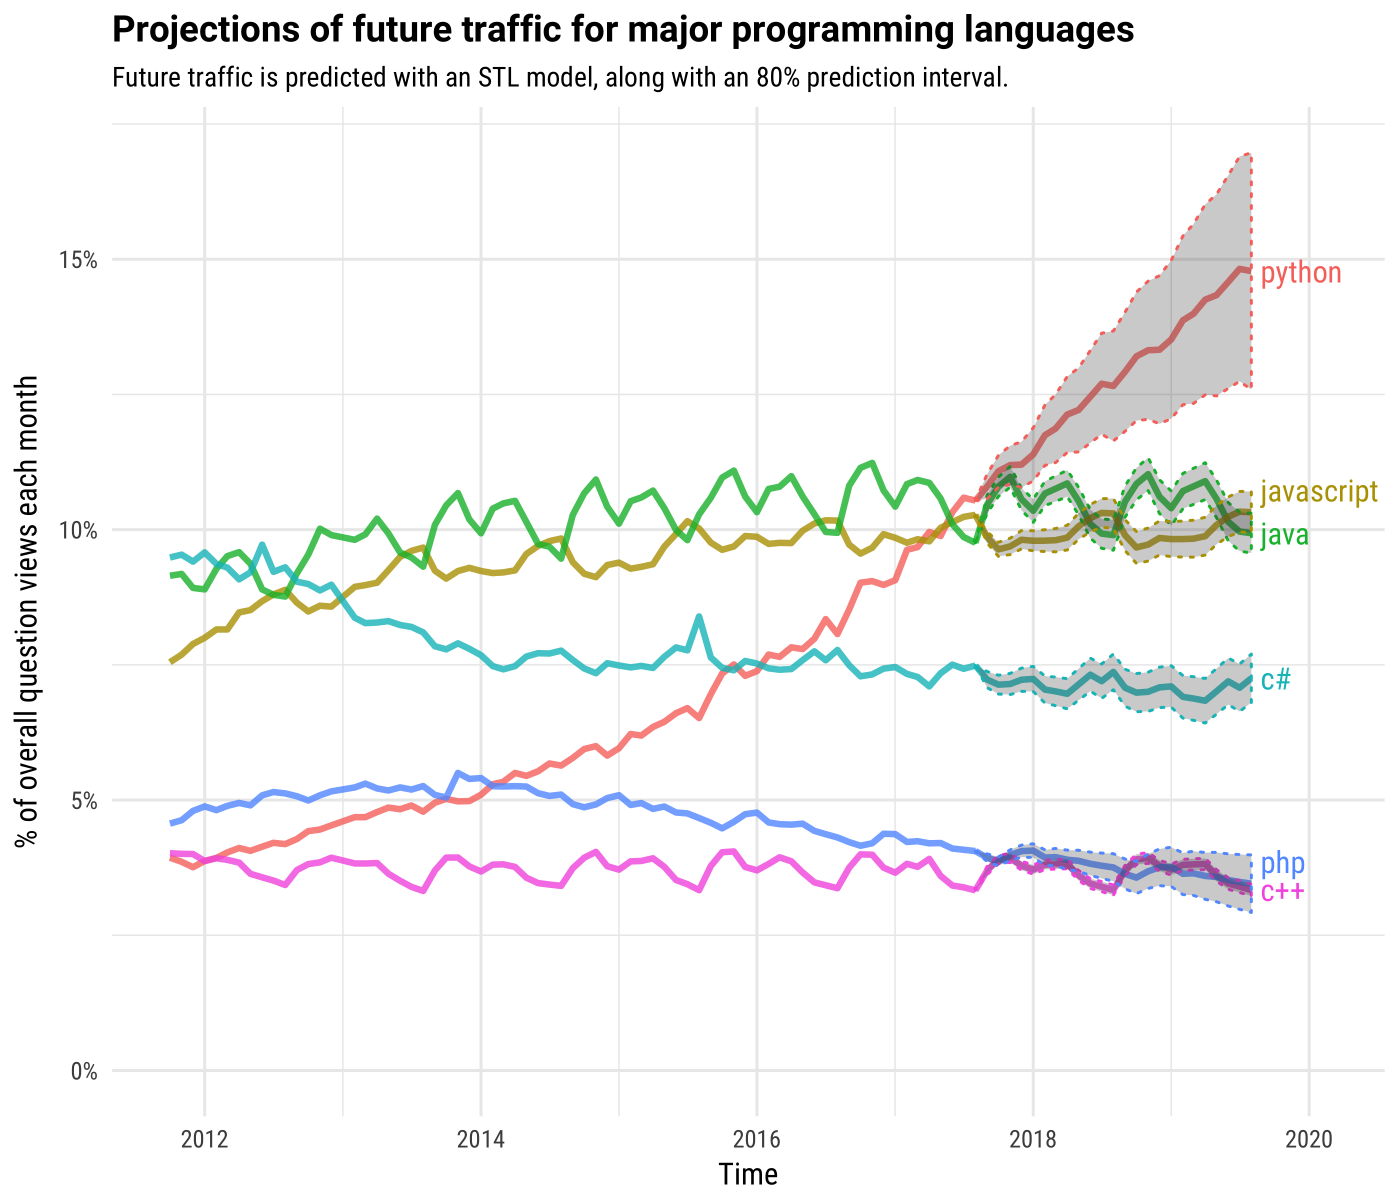
\includegraphics[width=\textwidth]{Figures/DataGeneration/projections-1-1400x1200.png}
    \caption{2018 projections of future internet traffic for major programming languages. Adapted from \cite{theoverflow}.}
    \label{fig:popularity}
\end{figure}


One of the reasons behind this tendency shift is the popularity of the language among machine learning and data science communities, fields where Python holds the first place by usage \cite{githubblog}. 
Since data-driven paradigms currently conform the state-of-the-art of many applied sciences, including audio signal processing, the availability of convenience Python packages and libraries is therefore of the highest interest to the research community. 

It is important to remark the predominant position that Matlab has always had regarding scientific computing. Indeed, it is still the tool of choice for many researchers, and the availability of libraries is accordingly very high. 
But the aforementioned tendency shift towards Python causes, as a side effect, the lack of many tools developed in Matlab by the research community.

Although Matlab code can be called and executed from Python, in practice this approach is suboptimal under several criteria. A better solution in the long run is the effective port of the code towards native Python code. Some of the libraries presented in this Chapter are partially or totally  motivated by this scenario.

	

\section{MASP: a Python library for multichannel acoustic signal processing}
\label{sec:masp}
\subsection{Description}

The Multichannel Acoustic Signal Processing (\textit{MASP}) is a Python library consisting of a collection of methods related with acoustics and microphone array processing.
The library is mostly a transcoding from several Matlab libraries by A. Politis\cite{politis2016microphone, github_politis}. 
It can be conveniently installed using \textit{pip}.

\textit{MASP} implements a variety of methods for the simulation and analysis of reverberant acoustic scenes, with emphasis on microphone arrays with spherical geometries.
More specifically, MASP is structured in submodules, with the following structure :

\begin{description}

	\item [Array Response Simulator] Simulation of
spherical microphones:
	\begin{itemize}
		\item Rigid/open configurations.
		\item Scattering simulation.
		\item Arbitrary capsule distances, positions and directivities.
	\end{itemize}
	
	\item [Shoebox Room Model] Fast implementation of the Image Source Method \cite{imagemethod}:
	\begin{itemize}
		\item Convex 3D rooms.
		\item Arbitrary number of sources and receivers, with arbitrary positions, orientations and directivities.
		\item ISM expansion limited by order or time.
		\item Frequency-dependent wall absorption.
		\item RIR with spherical harmonic expansion.
	\end{itemize}
	
	\item [Spherical Array Processing] Transformation and analysis of signals measured with a spherical microphone array:
	\begin{itemize}
		\item A2B conversion with theoretical or measured filters.
		\item Signal-independent beamforming.
		\item Signal-dependent and adaptive beamforming.
		\item Direction of Arrival estimation.
		\item Diffuseness estimation.
	\end{itemize}
	
	\item [Spherical Harmonic Transform] Mathematical convenience tools.
\end{description}

The library implements a Unit Testing system, which numerically assesses the validity of the methods. 
More specifically, each function test calls the equivalent Matlab code under the hood. The numeric result is then sent back to Python, where
it is evaluated against the own result.\\

Two example applications of the library are shown in Figures~\ref{fig:array_response} and \ref{fig:sht_filters}.
In Figure~\ref{fig:array_response} , obtained with the Array Response Simulator package, the frequency response of a spherical microphone array to an impinging plane-wave with varying incidence angle is shown. The microphone array consists of a 2nd order supercardioid and a 3rd order hypercardioid, located at opposite directions of an open sphere, and both of them facing to the front direction. \\

\begin{figure}[h!]
  \centering
    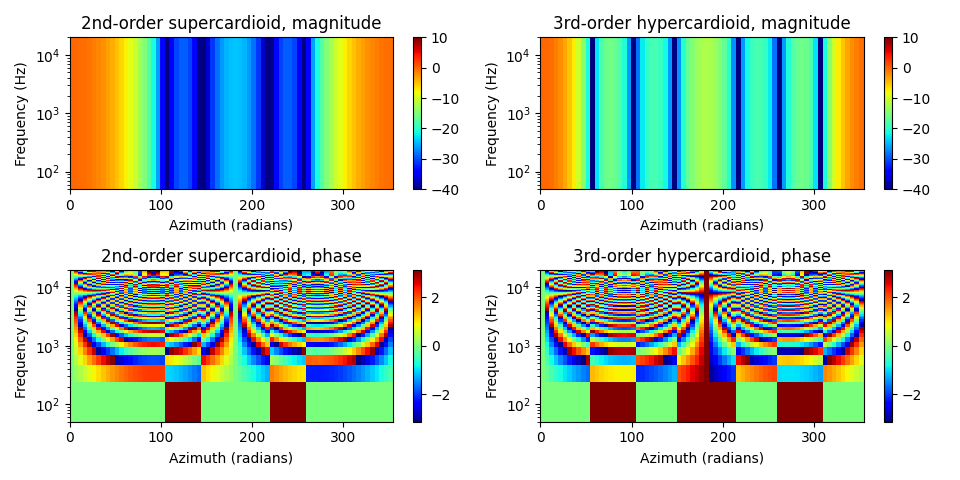
\includegraphics[width=\textwidth]{Figures/DataGeneration/array_response.png}
    \caption{Frequency response of an arbitrary spherical array.}
    \label{fig:array_response}
\end{figure}


One of the features of the Spherical Array Processing package is shown in Figure~\ref{fig:sht_filters}. The plot shows the evaluation of radial filters $\Gamma_n(kR)$ for an arbitrary spherical array, generated by inverting the theoretical response of the array \cite{Bertet2006}. 
The evaluation is performed following the metrics presented in the same paper, which compare spatial correlation, level difference and maximum amplification with respect to the ideal case. \\

\begin{figure}[h!]
  \centering
    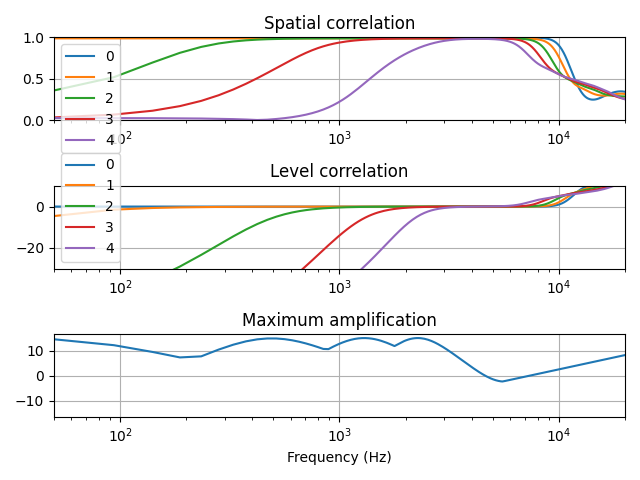
\includegraphics[width=1\textwidth]{Figures/DataGeneration/sht_filters.png}
    \caption{Evaluation of radial filters for an arbitrary spherical microphone array.}
    \label{fig:sht_filters}
\end{figure}

\subsection{Related software}

There exists another recent Python library which covers a similar scope: \textit{pyroomacoustics} \cite{scheibler2018pyroomacoustics}.
This framework provides an object-oriented interface with two main application scopes: allow RIR simulation of complex rooms based on the image source method, and provide a reference implementation of standard microphone array processing algorithms. 

Although some of the features are common to both libraries, there is a significant difference regarding their target usage. While \textit{MASP} primarily focuses on spherical geometries, \textit{pyroomacoustics} is more concerned about arbitrary room geometries and computational performance. 
Therefore, both libraries might be considered as complementary to some extent. 
A comparative list of their features is shown in Table~\ref{tab:masp_features}.



\begin{table}[th!]
\centering
\caption{Features of \textit{MASP} compared to \textit{pyroomacoustics}.}

\begin{tabular}{cccc}
  \toprule
Package & Feature &  MASP & PRA \\
\midrule
Shoebox & Convex 3D room         & \checkmark	& \checkmark \\
Room    & Non-convex 3D room     & -    			& \checkmark   \\
Model   & Arbitrary \#sources    & \checkmark   & \checkmark      \\
 & Arbitrary \#receivers, arrays & \checkmark   & \checkmark   \\
& ISM by max\_order                                 & \checkmark                              & \checkmark                              \\
& ISM by max\_time                                  & \checkmark                              & -                              \\
& Wall absorption                                   & \checkmark                              & \checkmark                              \\
& Frequency-dependent absorption                    & \checkmark                              & -                              \\
& Plot methods                                      & -                              & \checkmark                              \\
& RIR rendering                                     & \checkmark                              & \checkmark                              \\
& Audio simulation                                  & \checkmark                              & \checkmark                              \\
& Acoustic descriptor estimation                    & \checkmark                              & -                              \\
& Microphone orientation                            & \checkmark                              & -                              \\
& Custom microphone directivity                     & \checkmark                              & -                              \\
& RIR Spherical Harmonic Expansion                  & \checkmark                              & -                              \\

\midrule
Array   	& Rigid spherical arrays   & \checkmark                              & -     \\
Simulator 	& Arbitrary capsule geometries & \checkmark   & -  \\
           	& Recorded array IRs  & \checkmark                              & - \\
\midrule
Spherical & A2B conversion   & \checkmark      & -       \\
Processing  & Beamforming          		 & \checkmark      & \checkmark                              \\
 & Plane-wave decomposition         		 & \checkmark      & -                              \\
 & Nullformer                            & \checkmark      & -                              \\
& Adaptive Beamforming                   & \checkmark      & -                              \\
 & Adaptive Filtering             		 & -               & \checkmark                              \\
& DoA Estimation                         & \checkmark      & \checkmark                              \\
 & Diffuseness Estimation             	 & \checkmark      & -                              \\
 & Diffuse-field coherence               & \checkmark      & -                              \\
 & Blind Source Separation               & -               & \checkmark          \\                   
\bottomrule
 
\end{tabular}
\label{tab:masp_features}
\end{table}



\section{SOFA}

\subsection{Problem statement}

The availability of recorded room impulse responses is of great importance to many acoustic signal processing problems. 
Many different RIRs can be obtained from the same room, just by varying the position of the source and the receiver; when the number of source and receiver positions increases, the total amount of measurements increases geometrically. 
Besides that, the final format and organisation of the produced data (not only the RIR themselves, but also the source/position annotations) can be arbitrarily different when produced by different groups of people.

In order to overcome potential interoperatibility and reusability issues, the \textit{Spatially Oriented Format for Acoustics} (SOFA) convention \cite{majdak2013spatially}, also known as the \textit{AES-69} standard \cite{majdak2015aes69}, proposes a unified file format for the storage of IR-related data. 
Despite that SOFA was initially created with an emphasis on \textit{Head-Related Impulse Response} (HRIR) data, the framework that SOFA provides can be potentially applied to a variety of recording procedures and audio-related data. 
Such variety is associated with the concept of \textit{conventions}: a specific data structure designed to hold a concrete type of data or measurement. Some examples of widespread conventions might be \textit{SimpleFreeFieldHRIR} (for anechoic binaural measurements), \textit{SimpleHeadphoneIR} (intended for storing headphone impulse responses), or \textit{MultiSpeakerBRIR} (for binaural RIRs measured from loudspeaker arrays), to name a few of them.


\subsection{Ambisonics Directional Room Impulse Response as a SOFA convention}
\label{subsec:adrir}

Given the intrinsic spatial characterization capabilities of ambisonics, Gerzon proposed the technique as a potentially successful candidate format for acoustical heritage preservation, as early as 1975 \cite{gerzon1975recording}.

The increase in popularity of ambisonics since the beginning of the present century has turned this idea into reality; OpenAIRlib, a freely accesible dataset that gathers dozens of RIRs, might be a good example of it \cite{murphy2010openair, openair}.

In any case, the usage of recorded ambisonic RIRs is not limited to the field of acoustic heritage. Among others, the availability of such recordings has powered works in a variety of works, auralization \cite{postma2016virtual}, room acoustics analysis \cite{embrechts2015measurement,clapp2011investigations} and modelling \cite{romblom2017diffuse}, spatial audio synthesis \cite{coleman2017object} or source separation \cite{baque2016separation}. \\


In general, all publicly available ambisonic RIR measurements share some common approaches for describing and organizing the recorded data. 
For instance, recordings from different rooms are usually stored as separated folders. 
Each combination of emitter and receiver positions is often saved as an individual file, and the different spherical harmonics match the audio channels.
Moreover, it is also usual to provide a \textit{metadata} file, describing the different emitter and receiver positions, and potentially some information about the measurement setup, methodology, etc. Such files might be formatted as plain text or delimiter-separated files.
 
Despite the common approach, it can be easily foreseen that each database generated by a different individual or institution might potentially have a different naming convention, folder structure, file format, and so on. 
This is exactly the same situation that motivated the development of the SOFA conventions. 

On the other hand, the SOFA specification defines some criteria that must be fulfilled in order to propose a new convention \cite{sofaconventions}. These criteria are:
\begin{enumerate}
    \item Data must exist.
    \item Data can not be described by existing SOFA conventions.
    \item Relevant information about the data must be available.
\end{enumerate} 

Given that the described situation meets all requirements, the \textit{Ambisonics Directional Room Impulse Response} (AmbisonicsDRIR) convention has been therefore proposed as a new member of SOFA.\\

The technical specifications of the proposed convention in its current state (version 0.2) are available online \cite{ambisonicsdrir}. 
Despite a timid adoption of the convention, the AmbisonicsDRIR proposal has arisen interest in the community. At the moment of writing, the \textit{Standardisation Committee on AES-69 Standard} is discussing potential modifications to the SOFA file format required for the adoption of several new features; and the support for spherical harmonic-based measurements is among the topics for deliberation.


\subsection{Pysofaconventions}

The situation described in Section~\label{sec:intro_data}, regarding the availability of acoustic signal processing libraries in the Python programming language, can be easily extended to the case of SOFA APIs.
 
The library \textit{pysofaconventions} has been created with the aim to provide an alternative to the existing Matlab/Octave and C/C++ implementations. 
For ease of installation, it is integrated in the standard python package manager, \textit{pip}. 

The current software version is 0.1.5. The library structure is inspired by the C++ implementation \cite{api_cpp}. 
It features all functionalities described by SOFA version 1.0, plus the proposed AmbisonicsDRIR convention. 
The implementation is based on extensive error checking, to ensure code consistency.
 
\textit{pysofaconventions} has gained a moderate amount of attraction. Among others, it is being used as a dependency for the \textit{Real-Time Spherical Microphone Renderer (ReTiSAR) for binaural reproduction}, developed by Chalmers University in collaboration with Facebook Reality Labs \cite{helmholz2019real}. Furthermore, given the open nature of the project, several external researchers have contributed with bug fixes or new feature implementations.


\section{Ambiscaper}

%==================================================================

\subsection{Motivation}

The availability of data is a fundamental requirement for research. 
More specifically, in the scope of the B-Format data analysis in which this thesis focuses, audio is frequently generated on an IR-based manner, employing both acoustic simulations and recordings. 
%As already explained, the actual ambisonic audio under analysis is obtained from the convolution of the RIRs with any desired signal.
 In that way, the analysis can focus on different signal types, such as speech or music, usually employing dedicated external datasets. 

An alternative procedure for ambisonic data generation is the actual recording of sound scenes with spherical microphone arrays. 
Although this procedure might yield the most realistic sound field representations, the high cost, lack of scene control, and technical difficulty to obtain reliable groundtruth annotations lead to a limited usage of the technique, often reserved for real-life algorithm validation. 
%in two different ways: IR simulation and IR recording. As already explained, the actual ambisonic audio under analysis is obtained from the convolution of the RIRs with any desired signal. In that way, the analysis can focus on different signal types, such as speech or music, usually employing dedicated external datasets. 
 

%We may also consider a third type of B-Format audio generation, which is the actual recording of a sound scene. Although this procedure might yield the most realistic representation of the sound field, the high cost and lack of scene control leads to a limited usage of the technique, often reserved for real-life algorithm validation. 

It is of interest to have an insight of the diverse methods used in the literature for ambisonic sound generation. Table \ref{table:evaluationdata} summarizes the information gathered from works on the scope of sound source localization and separation, which have been published until 
2018\footnote{The original research to which this section refers was conducted in 2018, for the publication of \cite{perez2018ambiscaper}. Since then, the outbreak of localization-related challenges, such as LOCATA 2018 and specially DCASE 2019 and 2020, and the consolidation of data-based methods, has largely contributed to the homogenization of datasets \cite{evers2020locata, adavanne2019multi, politis2020dataset}. Still, most assumptions and results of our analysis continue to hold at present.}.
 The table displays, for each article, how the evaluation data was generated, and which was the type of audio content considered.
 

%% DOA ESTIMATION
\begin{table}[htpb]
    \centering
    \footnotesize

%	\begin{tabular}{ p{3cm} p{2.8cm} p{2.5cm} p{2.3cm} }
	\begin{tabular}{ ccc }
    \toprule
    % \cmidrule(r){1-2}
    
    % \centering 
    Article &
    % \textbf{\textit{$L$}} &
    Data Generation Method &
    Audio Content\\
    \midrule
    
    \cite{thiergart_localization_2009}
    % & 1 h
    & Audio recording 
    & Speech\\
    
    \cite{Tervo2009}
    % & 1 h
    & Audio recording
    & Noise, music\\
    
    \cite{Jarrett2010} 
    % & 4 
    & IR simulation, audio recording
    & Noise\\
    
    \cite{Nadiri2014}   
    % & 4 
    & IR simulation, audio recording
    & Speech\\
    
    \cite{Moore2015}   
    % & 4 
    & IR simulation 
    & Speech\\
    
    \cite{Pavlidi2015}
    % & 4
    & IR simulation 
    & Noise, speech\\
    
    \cite{He2017}   
    % & 1 h
    & IR simulation, audio recording
    & Speech\\
    
    % Ding \cite{Ding2017}   
    % % & 1 h
    % & IR simulation \& Audio recording \\
    
    \midrule
    
    \cite{Gunel2008}
    & IR recording
    & Speech, music\\
    
    \cite{Shujau2011} 
    & Audio recording
    & Speech\\
    
    \cite{Riaz2015}
    & IR recording
    & Speech, music\\
    
    \cite{Chen2015}
    & IR simulation, IR recording
    & Speech\\

    \bottomrule
    \end{tabular}
    \caption{Summary of audio data used across Ambisonics-based Source Localization (above) and Source Separation (below) methods.}
    \label{table:evaluationdata}
\end{table}

The statistics of the global usage of each generation method show that there is not a clear tendency towards any method.
Nevertheless, it is also noticeable that the methods with evaluations performed on real recordings make use of only one one sound scene in each case. In contrast, when using IR-based scenes, the number of audios evaluated are usually one or two magnitude orders greater. 

In addition, it is important to notice the lack of availability of the generated data. None of the analyzed articles provide a way to access neither the used audio dataset, nor the groundtruth (position annotations in the case of localization, and original sound sources for sound separation). 
Only when simulated IRs are used, it is possible to partially replicate the experimental setup --- the parameters used in the simulation software are usually provided. 
Furthermore, the process of dataset creation seems to be performed \textit{ad-hoc} in each case. 

Taking into account the flexibility offered by IR-based scenes, it would be desirable to have a tool for automatic generation of ambisonics scenes, and their associated annotations, for analysis purposes.
A tool with such characteristics would help the scientific community in several ways: (i) reducing the amount of time dedicated to build custom datasets, (ii) reusing publicly available resources and recordings, and (iii) enhancing experiment reproducibility by making easier the exchange of datasets. 
Moreover, the capacity of batch processing of large ambisonic collections might also contribute to the development of data-driven approaches.


\subsection{Implementation}
\label{sec:ambiscaper}

\textit{AmbiScaper} is a tool designed to provide a flexible way of creating complex ambisonics sound scenes and their associated groundtruth annotations, to be used in the context of source localization and separation algorithms.
\textit{AmbiScaper} offers a high level control of the sound scene parameters, and provides a simple interface for the creation of large datasets with custom characteristics.
\textit{AmbiScaper} is based on \textit{Scaper}, a framework designed to generate annotations for training Sound Event Detection models \cite{Salamon2017}.\\

One of the main features of \textit{AmbiScaper} is that all parameters of the sound scene can be specified in a non-deterministic way. In that sense, the parameters for each \textit{event} (sound source) are actually generated through a two-step process. First, in the \textit{Event Specification}, all parameters related to an event are defined in terms of statistical distributions. During the \textit{Event Instantiation}, the actual values for each parameter are then sampled from the statistical distributions.
This two-step process allows the user to describe abstract \textit{templates} of sound scenes, rather than manually assigning values to parameters. Therefore, a single \textit{event specification} might produce potentially infinite different sound scenes. \\


%%%%%%%%
In order to generate a sound scene, \textit{AmbiScaper} requires three different inputs: the original \textit{mono signals}, which will provide the actual audio content; an optional ambisonic RIR; and an \textit{event specification}. 

The process of dataset creation starts with the \textit{event instantiation}, as described above. Once all values are sampled, three different types of output are generated: the \textit{ambisonic scene}; the \textit{instantiated mono signals} (the original mono signals after data augmentation); and the \textit{annotations}, in the form of a \textit{jams} file \cite{humphrey2014jams}, containing all information about the instantiated values. 

The complete architecture of \textit{AmbiScaper} architecture is depicted in Figure~\ref{fig:architecture}.\\


\begin{figure}
  \centering
	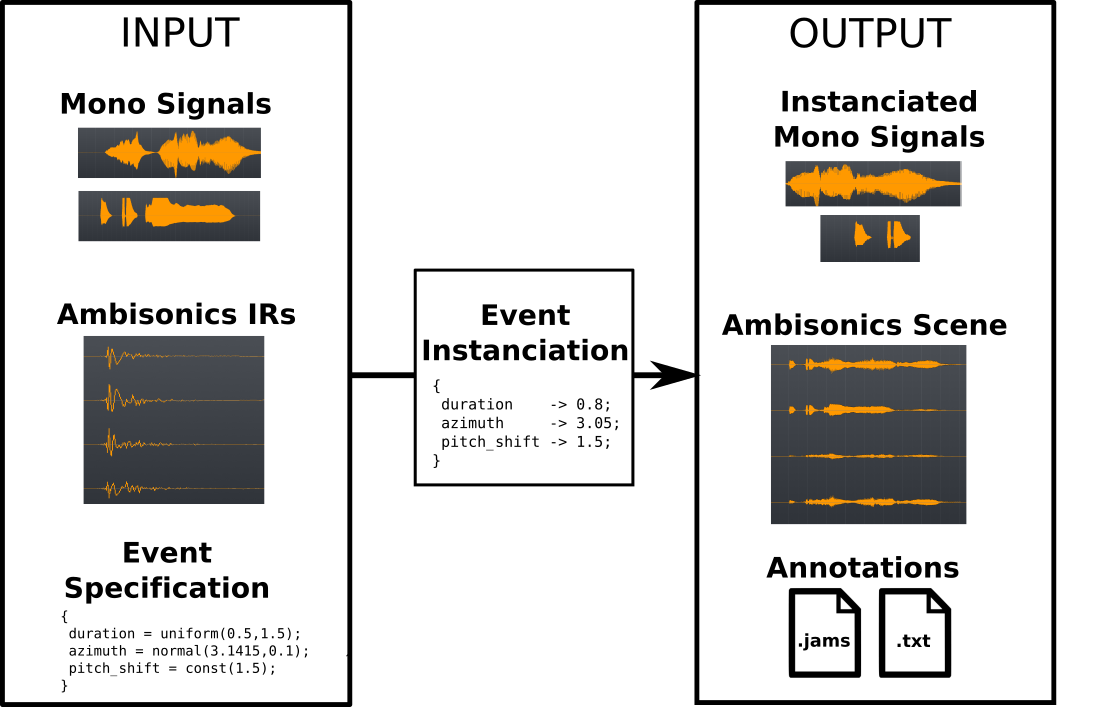
\includegraphics[width=\textwidth]{Figures/DataGeneration/figure_architecture_V2.png}
    \caption{\textit{AmbiScaper} architecture.}
	\label{fig:architecture}
\end{figure}



When no reverberation is specified, \textit{AmbiScaper} can generate anechoic sound scenes, using the theoretical expression of the ambisonic encoding as in Eq.~\ref{eq:encoding}.
In this case, there is no upper limit on the Ambisonics order of the rendered scene. 
Furthermore, the anechoic case allows the modification of the directivity of the source(s) through ambisonic order downgrade \cite{carpentier2017ambisonic}.

\textit{AmbiScaper} partially supports RIR-based scene creation. It features a limited set of recorded ambisonic IRs from the S3A database \cite{coleman2015s3a}; compatibility with the AmbisonicsDRIR (Subsection \ref{subsec:adrir}) could be easily included. On the other hand, the usage of simulated IRs is provided through a wrapper to the Matlab library \textit{SMIR Generator} \cite{smir}. In this case, the reverberation model specifications are defined as well in statistical terms, and the generated RIRs are also stored for evaluation purposes.



%\textit{AmbiScaper} features the possibility of using simulated Ambisonics IRs, through a wrapper to \textit{SMIR Generator}. In this case, the reverberation model specifications might be defined as well in statistical terms, and the generated IRs are stored for evaluation purposes. A working copy of Matlab is required to run this option.

%\textit{AmbiScaper} supports the usage of recorded Ambisonics IRs, although it is currently limited to IRs from the S3A database \cite{coleman2015s3a}. The development of a standardized file format for Ambisonics IRs, which is being discussed at the moment of writing, will provide the flexibility to work with arbitrary Ambisonics IRs.   
%
%Lastly, AmbiScaper features the possibility of using simulated Ambisonics IRs, through a wrapper to \textit{SMIR Generator}. In this case, the reverberation model specifications might be defined as well in statistical terms, and the generated IRs are stored for evaluation purposes. A working copy of Matlab is required to run this option.

%When a reverberant sound scene is created, the specific Ambisonics IRs used on the scene are also provided as an output. Other research problems such as dereverberation or room reflection modelling might therefore benefit from such data.
%



\subsection{Experiment reproducibility}

As already mentioned, there is a generalized lack of publicly available datasets of ambisonic reverberant sound scenes. 
Even when using general purpose audio/speech datasets, the actual evaluation data is usually not available.
In that sense, the potential compatibility of \textit{AmbiScaper} with public ambisonic RIR databases is a key aspect for reproducibility, since it would allow the systematic reutilization of acoustical measurements in the analysis context.

Furthermore, the output of the \textit{AmbiScaper} dataset generation process is not limited to the actual dataset. 
In fact, the resulting annotation file does not only contain the \textit{instantiation} (the actual values of each parameter in the sound scene), but also the \textit{specification} (the statistical distributions from which the instantiated values are sampled). 
In the scope of experiment reproducibility, the exchange of \textit{specification files} instead of actual audio files might greatly reduce the storage capacity and bandwidth required to transfer large databases. 

\textit{AmbiScaper} is implemented in the form of a Python package, and is publicly available through the \textit{Python Package Index} repository  under the GPL license, thus easing the software adoption and the potential engagement of the scientific community with the development. 

As an example of the potential capabilities of the software, a sample dataset for the evaluation of source localization algorithms has been created \cite{ambiscaperDataset}.
The dataset contains 300 FOA sound scenes, with a duration between 1 and 2 seconds, each one containing a number of static sound sources between one and three.
Sound sources might have different gains, and they are located at random positions around the sphere. 
The sources are randomly chosen from a subset of the Anechoic OpenAirlib database \cite{openair}, which mostly contains recordings from baroque musical instruments.
Reverberation is provided by the \textit{AudioBooth} recorded RIR from the S3A collection \cite{coleman2015s3a}.\\



\todo{explain current state, discussion, etc?}


%\subsection{Current state}
%
%
%
%
%AmbiScaper is a tool designed for easy dataset creation and exchange, in the context of reverberant Ambisonics Source Localization and Source Separation. It responds to the lack of public datasets for algorithm design, evaluation and reproducibility. An example dataset generated with AmbiScaper, and its analysis with state-of-the-art Source Localization algorithms are also provided.
%Further studies in Ambisonics IR position interpolation would allow creating non-static audio scenes, which might be an interesting feature. 
%Another feature in progress is the support for a standardized Ambisonics IR format \cite{perez2018ambisonics}, which will ease data reusability and provide the potential to cover a big variety of acoustic scenarios. 
%
%
%
%
%
%
%
